\chapter{Knowledge Graph Completion}
\label{cha:knowledge_graph_completion}

As discussed in section \ref{cha:knowledge_graphs} knowledge graphs are not complete. They contain noisy  and incomplete data. It is practically impossible to cover every possible entity and relation existing in the real-world or even in their domain. There might be missing entities and relations or a Knowledge Graph can include two entities/ relations representing the same real-world entity. Knowledge graph completion tries to tackle these and other problems. It can be seen as a way of data cleaning and expansion for knowledge graphs. In the following three examples are given for knowledge graph completion tasks:

\textbf{Entity Resolution} is according to Talburt "the process of determining whether two [entities] are referring to the same object or to different objects". \cite{talburt_entity_2011} \\ 

\textbf{Entity Prediction} is the task of integrating new entities into the knowledge graphs. These entities are are discovered from other external sources and the knowledge graph includes no information about them. The goal is to find all possible relations this new entity has to the entities already existing in the graph. \cite[p.~1]{baumgartner_entity_2021} \\

\textbf{Link Prediction} is quiet similar to entity prediction. Instead of finding links for a new entity the goal here is to find all missing relations between already existing entities. \cite[p.~125]{golbeck_analyzing_2013} Link prediction can be approached in two different ways: entity classification and triple classification. "Entity classification tries to predict the type or the class of an entity [...]" \cite{ilkou_symbolic_2020} For a triple with a missing tail $(h,r,?)$ the goal would be to list all entities which fit into the tail along with their confidence. Triple classification on the other hand is a binary tasks. Here the input is a compete triple $(h,r,t)$ and the goal is to predict whether this triple is true or not. \cite{ilkou_symbolic_2020} \\

In the following we are going to focus on the task of link prediction. There are various models tackling the task. They can be categorized into one of the following two categories: symbolic and sub-symbolic approaches. Symbolic approaches try to reason about the problem with logic, this makes them comprehensible for humans. Sub-symbolic approaches on the other hand, solve the problem through less explainable mathematical equations. \cite{ilkou_symbolic_2020}

\section{Symbolic Approaches}
\label{cha:symbolic_methods}
Symbolic approaches, or also sometimes referred to as "Good Old Fashioned Artificial Intelligence", focus on learning hypothesises in a symbolic (logical) language. \cite{hogan_knowledge_2021} The strength of models from this approach lies in their explainability. Since the learned hypothesis are expressed in a logical language, either as axioms or rules, they are interpretable for a human and we can therefore reason about their predictions. In the following we will focus on rule-based models because they are more present for the link prediction task.  \cite{hatzilygeroudis_neuro-symbolic_2005} 
Rules are basically if-then clauses. Each rule has one or more conditions which have to be true and if they hold true the rule "fires" and its conclusion can be derived. They are often written down as Horn clauses, an example for a Horn clause can be seen in its disjunctive and implicative form in equation \ref{eq:horn_disjunct} and \ref{eq:horn_implic} respectively. \cite{chandra_horn_1985}

\begin{equation}
\label{eq:horn_disjunct}
A \wedge \neg B_1 \vee \neg B_2 \vee ... \vee \neg B_n \end{equation}

\begin{equation}
\label{eq:horn_implic}
A \leftarrow B_1, B_2, ..., B_n
\end{equation}

Both equations express the same clause which states that if all conditions $B$, also called body atoms, are true so is the conclusion $A$, which is also referred to as the head.

\subsection{AnyBURL}
\label{cha:anyburl}
AnyBURL \cite{meilicke_anytime_2019}, short for Anytime Bottom-Up Rule Learning, is a link prediction algorithm that generates a set of rules from an existing knowledge graph and leverages the generated rules to make predictions. The core idea behind AnyBURL  is that "[...] sampled paths from a knowledge graph (random walks) are examples of very specific rules, which can be transformed into more general rules." \cite{ott_safran_2021} 

\subsubsection{Rule Generalization}
\label{cha:anyburl_generalization}
Rules are learned bottom-up, meaning we start with a sampled random path in the knowledge graph which then gets generalized into a rule. The sampled random path is called the ground path or grounding. In \cite{meilicke_anytime_2019} generalized rules are classified into three types $AC_1$, $AC_2$ and $C$. 

$C$ rules are generalizations of cyclic 
ground paths:

\begin{equation}
h(Y,X) \leftarrow b_1(X, A_2), ..., b_n(A_n,Y).
\end{equation}

$AC_2$ rules are generalizations of acyclic ground paths:

\begin{equation}
h(c_0,X) \leftarrow b_1(X, A_1), ..., b_n(A_n,A_{n+1}).
\end{equation}
	
$AC_1$ rules can be generalized from both cyclic (with $c_0=c_{n+1}$) and acyclic ones ($c_0\neq c_{n+1}$):

\begin{equation}
h(c_0,X) \leftarrow b_1(X, A_1), ..., b_n(A_n,c_{n+1}).
\end{equation}

$X$ and $Y$ are for variables appearing in the head of the Horn clause, $A_i$ is a variable appearing only in the body and $c_i$ is a constant. Furthermore, $h(e_1,e_2)$ and $b_i(e_1,e_2)$ are another notation to express a triple $(e_1, h, e_2)$ or $(e_1, b_i, e_2)$. 

To get from a randomly sampled path to a rule a generalization lattice is build. The root of this lattice is the randomly sampled path and from there it is step-wise modified by either of the two following operations: 

\begin{enumerate}
\item all occurrences of a constant are replaced by a new variable 
\item an atom of the body is dropped
\end{enumerate}

After applying one of these a operations, the resulting rule is put into one of the following three categories:

\begin{enumerate}
\item Ambiguous Prediction
\item Shorter Bottom Rule
\item Useless Atom 
\end{enumerate}

Ambiguous predictions have a variable in the head which does not appear in the body of the rule. Therefore the rule does not make a concrete prediction and is not useful for the task of link prediction. Shorter bottom rules are rules which might be useful but can also be deprived from the generalization lattice of a shorter path. To avoid duplicates, rules are only created from the shortest path. The last category, useless atom, is the only one which gets generalized further. Rules fitting into this category have either an atom with only constants or an atom with a constant and an unbound variable. A unbound variable is a variable not appearing in any other body atoms or the head. 

If a rule does not fit into either of these categories it is a fully generalized rule and can be added to the final set of rules. In figure \ref{fig:generalization_lattice} an example of a generalization lattice for an acyclic path can be seen. \cite{meilicke_reinforced_2020}

\begin{figure}[H]
\centering
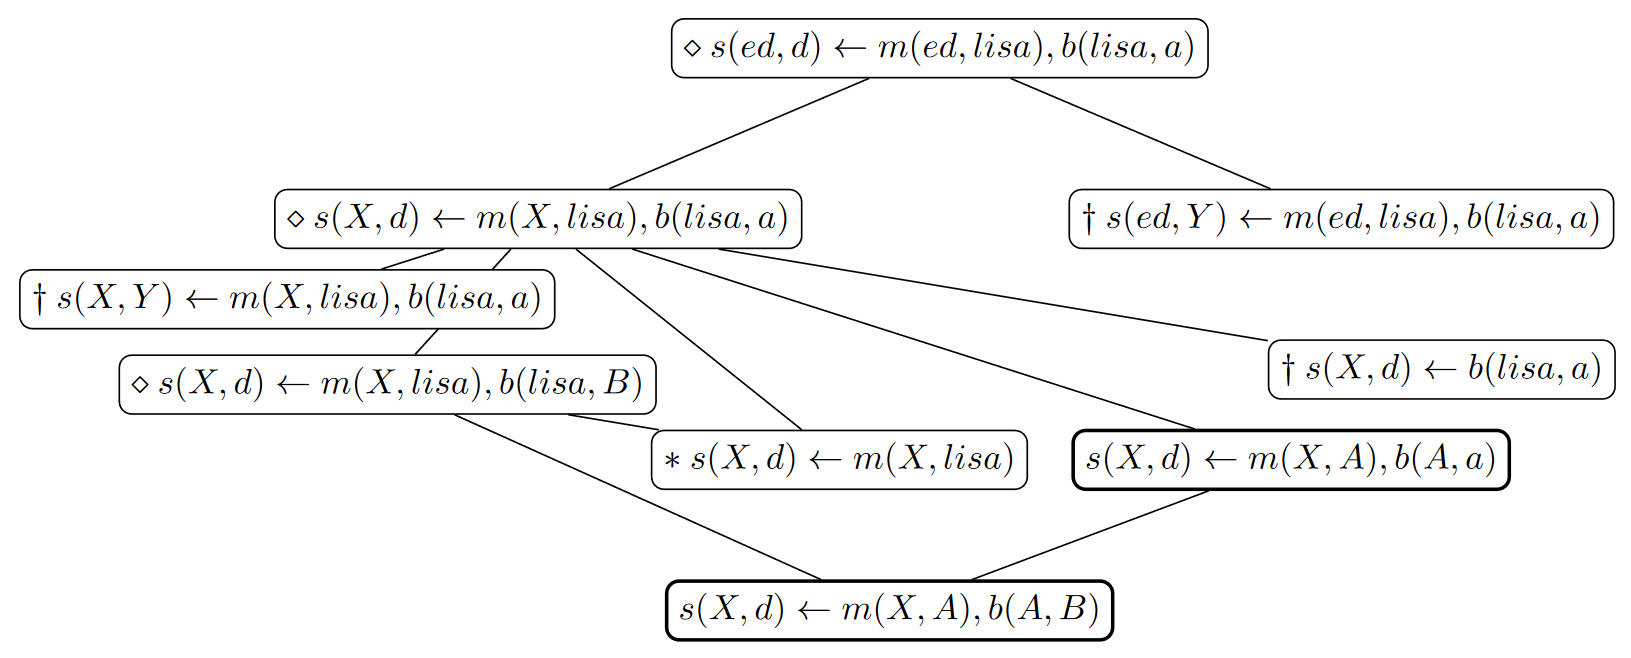
\includegraphics[width=0.9\textwidth]{images/example_generalization_lattice.png}
\caption{Example of a generalization lattice of an acyclic path (Ambiguous Prediction $\cross[.4pt]$, Shorter Bottom Rule $\ast$, Useless Atom $\diamond$)}
\label{fig:generalization_lattice}
\end{figure}

The lattice starts with the path $s(ed,d) \leftarrow m(ed,lisa), b(lisa,a)$ through applying the the generalization operations to final rules are created, the $AC_1$ rule $s(X,d) \leftarrow m(X,A),b(A,a)$ and the $AC_2$ rule $s(X,d) \leftarrow m(X,A),b(A,B)$.

In \cite{meilicke_reinforced_2020} it is argued that those two rules are always the result if an acyclic path is generalized and therefore AnyBURL does not need to build the entire generalization for every sampled path but can directly create these rules. The same goes for cyclic path. A generalization will always lead to a $C$ and two $AC_1$ rules.   

\subsubsection{Rule Learning}
\label{cha:anyburl_learning}
Algorithm \ref{alg:anyburl} shows the AnyBURL algorithm for learning rules. AnyBURL learns rules by sampling random paths of the length $n$ and generalizes these to rules as discussed in the previous section. The function $score(r,s)$ computes the confidence of rule efficiently by using a sampling strategy, where the parameter $s$ specifies the sample size. The confidence can then be used to check whether the quality criteria $Q$ is satisfied. In case it is satisfied, the rule is added to the final set of rules and otherwise discarded. The algorithm tries to find as many rules as possible within the time frame $ts$. Afterwards it checks if the current amount of rules for paths of the length $n$ satisfy a certain saturation $sat$. If it does $n$ is increased and if not another timeslot of the length $ts$ is spend searching further rules of the same length. \cite{meilicke_anytime_2019}

\begin{algorithm}[H]
\caption{Anytime Botton-up Rule Learning}
\label{alg:anyburl}
\begin{algorithmic}[1]
\STATEx AnyBURL($\mathbb{G},s,sat,Q,ts$)
\STATE $n=2$
\STATE $R=\emptyset$
\LOOP
\STATE $R_s=\emptyset$
\STATE $start=currentTime()$
\REPEAT
\STATE $p=samplePath(\mathbb{G},n)$
\STATE $R_p=generateRules(p)$
\FOR{$r\in R_p$}
\STATE $score(r,s)$
\IF {$Q(r)$}
\STATE $R_s=R_s \cup \{r\}$
\ENDIF
\ENDFOR
\UNTIL{$currentTime()>start+ts$}
\STATE ${R'}_s = R_s \cap R$
\IF {$|{R'}_s|/|R_s|>sat$}
\STATE $n=n+1$
\ENDIF 
\STATE $R=R_s \cup R$
\ENDLOOP
\STATE \textbf{return} $R$
\end{algorithmic}
\end{algorithm}

\subsubsection{Rule Application}
If the algorithm from the previous section is applied to a knowledge graph it returns a set of rules $R$. These rules can then be used to create a ranking of candidates to fill in an incomplete triple $(h,r,?)$ or $(?,r,t)$. In \cite{meilicke_anytime_2019} two methods are proposed to calculate this ranking of candidates. 
The first method is refereed to as Noisy-Or and calculates the confidence of a candidate by multiplying the confidences of all rules applicable to the candidate. 
The second method orders the candidates based on their rule with the highest confidence. In case two candidates got the same confidence, they are ordered by their second best rule and so on, until all candidates are ordered. 
The first method assumes that all rules are independent, while the second method ranks candidates, for which two independent rules fire, too low. 

In the paper it is discussed that the independence assumption is often wrong and therefore it makes more sense to apply the second method. They also provide numbers which support this assumption. 

\section{Sub-Symbolic Approaches}
\label{cha:sub_symbolic_methods}

Sub-symbolic approaches are based on statistics. They try to learn numerical models from the existing facts in the knowledge graph. These models can then be used to predict the existence of a triple.  \cite{nickel_review_2015} The most prominent models for knowledge graph completion of this approach are embedding-based models. These models learn a vector representation for each entity and relation. This is also often referred to as an embedding. In this representation it is then assumed that similar entities and similar relations will have similar vectors. An example for these embeddings can be seen in figure \ref{fig:embedding_example}. On the left side we see a knowledge graph with three entities and two relations. Every entity and relation are represented on the right side by an embedding. Our two entities \textit{Washington D.C} and \textit{New York City} are both cities and therefore we can assume that their semantic meaning are quiet similar. The embeddings of these two entities are also quiet similar which demonstrates that our previous assumption is correct. \cite{bianchi_knowledge_2020} Our embeddings are also called latent features because they can not be directly observed in the data. Instead our model has to infer these features from the data. \cite{nickel_review_2015} 

\begin{figure}[H]
\centering
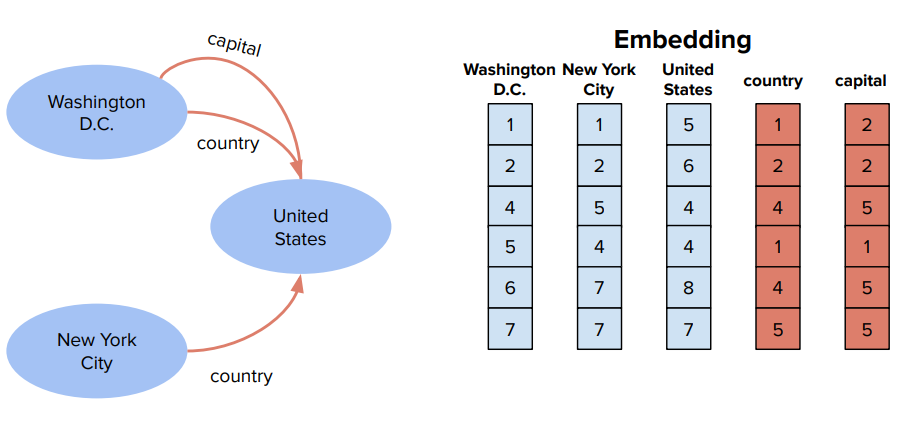
\includegraphics[width=0.9\textwidth]{images/embedding_example.png}
\caption{Example of an Embedding for a Knowledge Graph}
\label{fig:embedding_example}
\end{figure}

An embedding-based model is defined by three characteristics \cite{bianchi_knowledge_2020}:

\begin{enumerate}
\item representations of entities and relationships
\item the scoring function
\item the loss function
\end{enumerate}

As stated earlier our entities and relations are represented through vectors, their embeddings. Some models vary from this a bit and use complex numbers instead of real ones \cite{trouillon_complex_2016}  or use matrices to represent relationships \cite{nickel_three-way_2011}.

The score function $f(h,r,t)$ calculates the distance between the embeddings of two entities relative to their relation. If the triple holds true, its score should be in an optimal case equal to $1$. 
Lastly the loss function defines the objective which is going to be minimized during the training of our model where the embeddings for our entities and relations are learned. 
After learning the entity and relation representations through optimizing the loss function for the given score function, the model can be used to create a ranking of all candidates for a triple missing either its head $(?,r,t)$ or its tail $(h,r,?)$. The score is then calculated for all candidates $c \in C$ such that $(c,r,t)$ or $(h,r,c)$ do not exists in the given knowledge graph. All candidates are then sorted by their score which then results in the ranking. 

\subsection{RESCAL}
\label{cha:rescal}
One such an embedding-based model is RESCAL \cite{nickel_three-way_2011}\cite{nickel_factorizing_2012}. The model explains triples via pairwise interactions of latent features. It calculates the score of a triple as

\begin{equation}
\label{eq:rescal_score}
s(h,r,t)=e_h^T M_r e_t
\end{equation}

where $e_h, e_t \in \mathbb{R}^D$ and $M_r \in \mathbb{R}^{D*D}$. In this formula the interactions between two entity vectors are captured using only multiplicative terms, which makes this a bilinear model.

Furthermore, we can see that entities are encoded into a $D$-dimensional vector representation and have the same representation regardless of whether they occur as head or tail entity in a triple. Moreover, they also share the same representation for entities independent of the relation in a triple. Meaning that for every relation the vector of an entity stays the same. In \cite{nickel_review_2015} the authors of the RESCAL model argue that this allows their model to "[...] propagate information between triples [...]" and "[...] capture global dependencies in the data.". The relation in equation \ref{eq:rescal_score} is represented via a matrix $M_r$. Important to note about this matrix is its asymmetry. This allows the model to capture asymmetric relations e.g. while the model should predict the triple $(Darth\_Vader,$ $ father\_of,$ $Luke\_Skywalker)$ as \textit{True}, the triple $(Luke\_Skywalker,$ $ father\_of,$ $ Darth\_Vader)$ should be predicted as \textit{False}. 

\subsubsection{Training through RESCAL-ALS}
The model is trained through finding estimates for the matrices $E$ and $M_r$ which can be achieved by solving following regularized minimization problem

\begin{equation}
\label{eq:rescal_min_problem}
\min_{E, M_r} f(E,M_r) + g(E, M_r)
\end{equation}

where 

\begin{equation}
\label{eq:rescal_als}
f(E,M_r)=\frac{1}{2}(\sum_{h,r,t} \norm{X_{hrt}-s(h,r,t)}^2_F)
\end{equation}

and 

\begin{equation}
\label{eq:rescal_regu}
g(E, M_r)=\frac{1}{2}\lambda(\norm{E}^2_F + \sum_k\norm{M_r}^2_F).
\end{equation}

The term $g$ is included as regularization term to prevent the model from overfitting. The regularized minimization problem in equation \ref{eq:rescal_min_problem} is solved with an for RESCAL adjusted version of the alternating least-squares approach called RESCAL-ALS. This approach consists of a sequence of very efficient, closed-form updates as described in \cite{nickel_factorizing_2012}. This training method assumes the closed-world assumption.

\subsubsection{Training through Pairwise Loss}
In \cite{nickel_review_2015} an alternative training method under the open-world assumption is presented which is more similar to the way other embedding-based models are trained. They refer to it as pairwise loss. Here two sets of triples are used to train the model, positives and negatives denoted as $D^+$ and $D^-$ respectively. The positive triples are every known existing triple in our knowledge graph and the negative triples are created by corrupting existing triples. For the triples in the negative set it is not guaranteed that they are negative since a randomly corrupted triple could actually be an unknown true fact, but they are seen as \textit{assumed-to-be-negative}.

Using stochastic gradient descent or any of its variations following objective function is then minimized 

\begin{equation}
\label{rescal_pairwise}
\min_{E,M_r} \sum_{x^+ \in D^+} \sum_{x^- \in D^-} \mathcal{L}(s(x^+), s(x^-)) + g(E, M_r)
\end{equation}

using the same regularization as in equation \ref{eq:rescal_regu} and where $\mathcal{L}$ is a margin-based ranking loss function such as

\begin{equation}
\label{eq:rescal_loss}
\mathcal{L}(s,s') = max(1+s'-s,0).
\end{equation}
 
The usage of the margin-based loss has the advantage that negative triples do not have to be necessarily negative, they just have to be "more negative" than the positive ones. 

\subsection{DistMult}
\label{cha:distmult}
DistMult \cite{yang_embedding_2015} is another embedding-based model. It also uses the same basic bilinear scoring function as RESCAL in equation \ref{eq:rescal_score}. The difference here is that DistMult restricts the relation matrix $M_r$ to be a diagonal matrix. This reduces the parameters for the learnable parameters for a single relation from $D*D$ to just $D$. Therefore DistMult can be seen as a simplified version of RESCAL with the score function

\begin{equation}
\label{eq:distmult_score}
s(h,r,t)=e_h^T diag(r) e_t
\end{equation}

where $e_h, e_t$ and $r\in \mathbb{R}^D$. The reduction of the relation dimensionality makes the model more computational efficient, especially on large knowledge bases, but also less expressive than RESCAL. Chen \cite{chen_knowledge_2020} provides a good graphic to compare the two models which can be seen in figure \ref{fig:rescal_distmult}.

\begin{figure}[H]
\centering
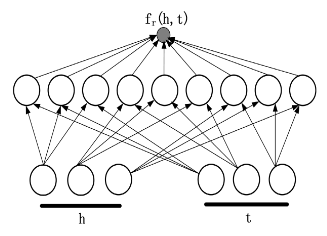
\includegraphics[width=0.45\textwidth]{images/rescal.png}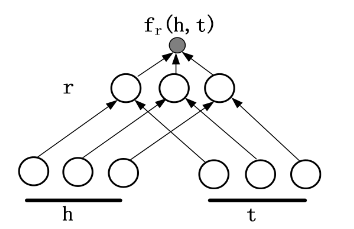
\includegraphics[width=0.45\textwidth]{images/distmult.png}
\caption{RESCAL vs. DistMult}
\label{fig:rescal_distmult}
\end{figure}

Here our dimension size is $D=3$. As we can see in RESCAL this leads to us having $3^2$ latent features for the relation which have to be learned during the training while DistMult requires only $3$.

\subsection{ComplEx}
\label{cha:complex}
While DistMult is more effective in regard to time and space complexity, it can not express antisymmetric relations. RESCAL on the other hand can express this but the size of the relation matrix leads to an explosion in the number of parameters. 
To combine the advantages of both methods Trouillon proposes a model called ComplEx  \cite{trouillon_complex_2016}. ComplEx uses a similar score function as DistMult but instead of calculating the dot product between the embeddings as real numbers, it uses complex vectors to represent the entities and relations. The dot product of complex vectors is referred to as the Hermitian dot product. Other than the dot product of real numbers it is not symmetrical. This enables the model to capture asymmetric relations while retaining the efficiency benefits of DistMult. The score function of ComplEx is 

\begin{equation}
\label{score_complex}
s(h,r,t)=Re(<w_r,e_h,\bar{e}_t>)
\end{equation}

where $e_h, e_t$ and $w_r\in \mathbb{C}$. To use this score function in our loss function, as defined in equation \ref{eq:rescal_loss}, the resulting scores need to be purely real. Therefore after calculating the Hermitian dot product only the real part is kept and the imaginary part simply discarded.  

\subsection{ConvE}
\label{cha:conve}
ConvE \cite{dettmers_convolutional_2018} presents another model trying to solve the task of link prediction. This model differentiates itself from other models by using 2D-convolutions over their embeddings. They argue that the use of a 2D convolution creates additional points of interaction between the embeddings and therefore increase the expressiveness of their model. 

Convolution modifies an input by a filter. The filter has to have the same amount of dimensions as the input. Therefore if we have an 1-dimensional input we have to either use 1D-convolution or transform our input into a higher dimensional representation. Figure \ref{fig:example_conv} depicts an example of how a convolution filter is applied in a two dimensional space. This example has a filter of the size $3 \times 3$. A feature map is calculated by multiplying the input with the filter. Here the first element of the input is multiplied with the first element of the filter, then the second with the second and so on. To calculate the next feature map the filter would be shifted one to the right and the same process would be repeated until the filter reaches the end of the input. Filters are also often referred to as kernel and can have different sizes. \cite{zhang_parallel_1990}

\begin{figure}[H]
\centering
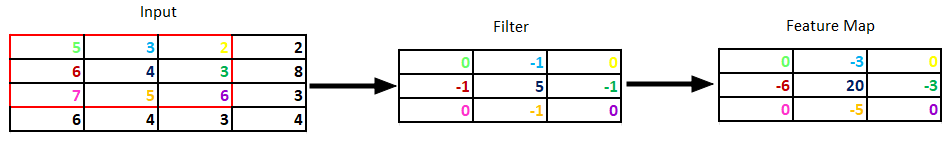
\includegraphics[width=0.9\textwidth]{images/convolution_filter_example.png}
\caption{Example of a Convolution Filter}
\label{fig:example_conv}
\end{figure}

In the following I will explain how ConvE integrates the convolution into their model along figure \ref{fig:conve}. In the beginning the embedding of the head entity $e_h \in \mathbb{R}^k$ and of the relation $r_r \in \mathbb{R}^k$ are reshaped into 2D $\bar{e_s},\bar{r_r} \in \mathbb{R}^{k_w \times k_h}$, where $k=k_wk_h$.
The two reshaped embeddings are then concatenated and used as an input for a 2D convolution with filters $\omega$ of the size $m \times n$.
The resulting feature maps are then transformed into a vector $vec \in \mathbb{R}^{c \times m \times n}$ where $c$ is the number of features maps generated from the convolution. 
In the next step the vector is projected into a k-dimensional space using linear transformation parametrized by the matrix $W \in \mathbb{R}^{cmn} \times k$. Finally the inner product between the projected vector and the embedding of the tail entity $e_t \in \mathbb{R}^k$ results in the final prediction. \cite{dettmers_convolutional_2018}

\begin{figure}[H]
\centering
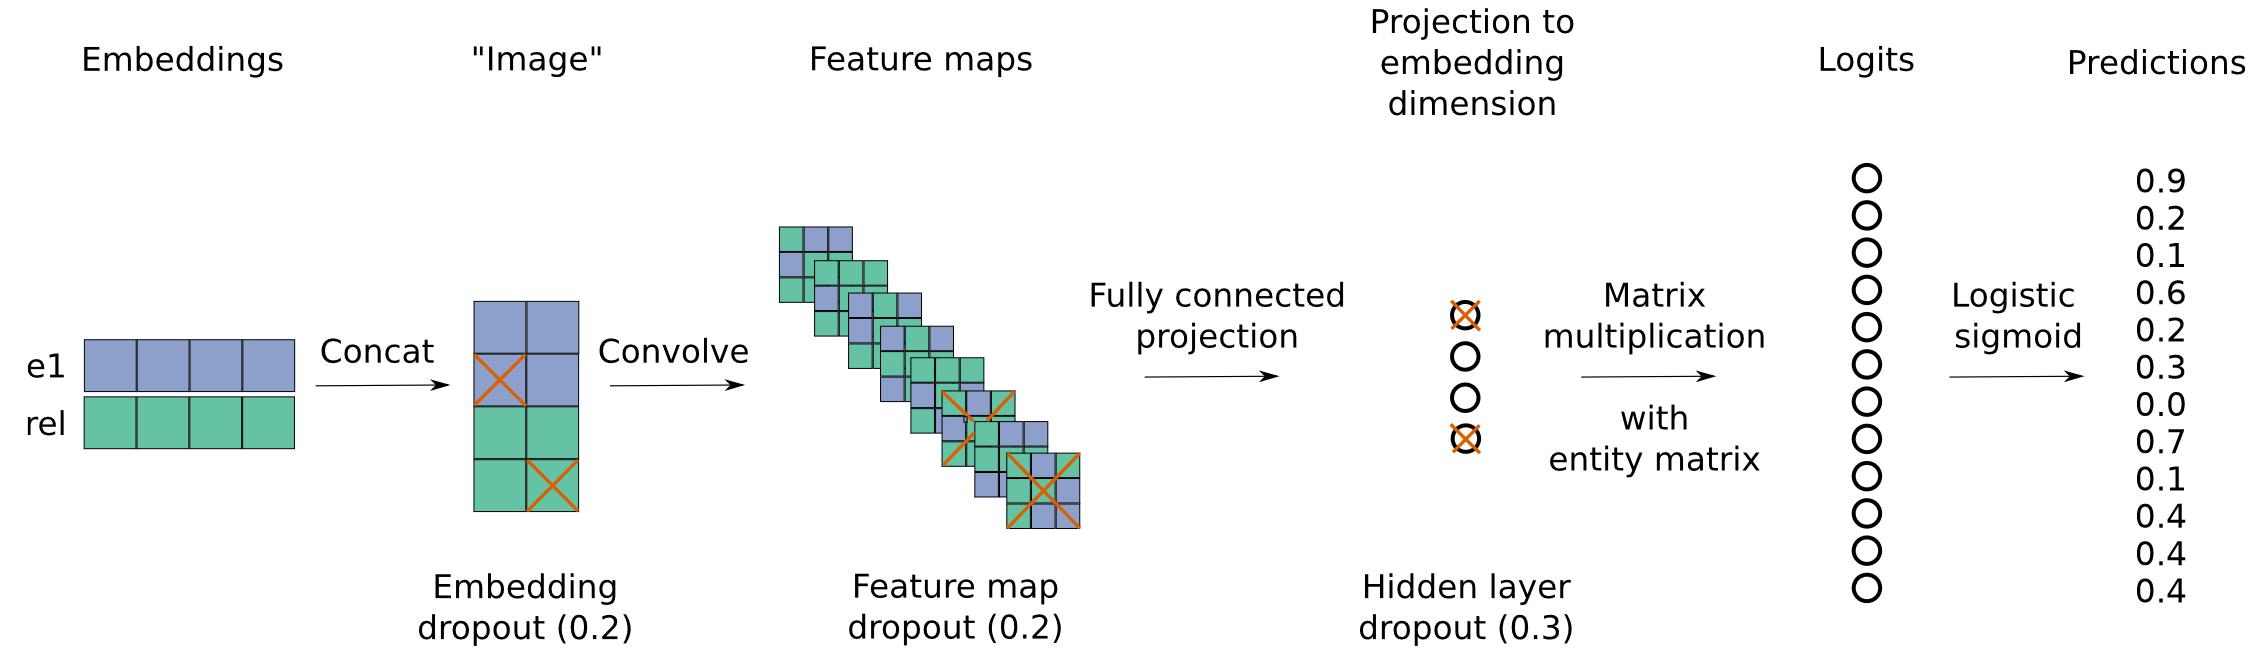
\includegraphics[width=0.9\textwidth]{images/conve.png}
\caption{Steps of the ConvE Model}
\label{fig:conve}
\end{figure}

Formally the above can be defined as the score function of the model:

\begin{equation}
s(h,r,t)=f(vec(f([\bar{e_h};\bar{r_r} * \omega))W)e_t
\end{equation}

Furthermore, the authors of the model suggest using a different loss function. Instead of the margin-based loss RESCAL, DistMult and ComplEx are using, ConvE uses binary cross entropy loss: 

\begin{equation}
\mathcal{L}(s,s') = s'*log(s)+(1-s')*log(1-s))
\end{equation}

\section{Comparison of the Approaches}
\label{cha:compare_approaches}
In the previous sections symbolic and sub-symbolic models have been presented. In the following we have a deeper look into the differences in terms of advantages/ disadvantages of these two approaches.

The main advantage for the symbolic approach as previously mentioned is the explainability. Especially in a rule-based system results and often intermediate steps can be directly explained and it can be shown which part of the data lead the model to its results. In real world applications having a result which can be explained is often a wanted feature and sometimes it might also become mandatory through laws such as the European Union’s General Data Protection Regulation. A sub-symoblic model does not offer the possibility of an explanation for its results. 

A further advantage of rule-based models is the possibility to modularly adjust the rules. Rules can be added or removed at any given time. A sub-symbolic model on the other hand has to be completely retrained once the trainings data changes and its impractical to make small adjustments to trained parameters. This modularity rule-based systems offer also allows for a knowledge transfer between different models. Rules from one model could be copied into the other. 

Sub-symbolic approaches on the other side are often easier to scale up and therefore can be better applied to larger knowledge bases. The models are often computational more efficient but have a large amount of hyperparameters which have to be optimized. Moreover, embedding-based models are robuster to noisy or missing data, compared to rule-based models, since rule-based models derive rules from specific facts where embedding-based models only use the facts as one under many to optimize its parameters. This on the other hand makes the embedding-based models more dependent on the distribution of the trainings data. If the trainings data only contains a few examples for a entity or relation the parameters are likely to not be optimized for this entity or relation in favour of being better in predicting an entity or relation more frequently represented in the data. \cite{ilkou_symbolic_2020}


\section{Model Evaluation}
\label{cha:evaluation}
As discussed in section \ref{cha:symbolic_methods} and \ref{cha:sub_symbolic_methods} both methods are used to generate a ranking of candidates for an incomplete triple $(h,r,?)$. As the rank of such an triple one understands the position at which the correct answer is in this ranking. This is also often refereed to as the raw rank. The rank can be filtered by other known true triples which is then called the filtered rank i.e. when evaluating the predictions for a triple $(h,r,t)$ there might be other triples in the knowledge graph $(h,r,t')$ for $t \neq t'$, since $(h,r,t')$ exists in the knowledge graph and therefore is also a true triple it is desirable to give it a high score and a low rank. This could affect the rank of the triple $(h,r,t)$ in a negative way. To avoid this other true triples are not counted for the filtered rank. Therefore the filtered rank is always less or equal to the raw rank. \cite{bordes_translating_2013}

In most cases when evaluating a link prediction model a test dataset is given which includes a set of prior unknown triples for which the head and tail are predicted. The resulting ranks can then be used to calculate one or more of the following metrics in order to compare the general performance of different models: Hits@k (eq. \ref{eq:hitsk}), Mean Rank (eq. \ref{eq:mr}) and Mean Reciprocal Rank (eq. \ref{eq:mrr}). 

\begin{equation}
Hits@k=\frac{|{q \in Q | rank(q) \le k}|}{|Q|}
\label{eq:hitsk}
\end{equation}

\begin{equation}
MR=\frac{1}{|Q|} \sum_{i=1}^{|Q|}{rank_i}
\label{eq:mr}
\end{equation}

\begin{equation}
MRR=\frac{1}{|Q|} \sum_{i=1}^{|Q|}{1/rank_i}
\label{eq:mrr}
\end{equation}

with $Q$ being the set of test triples. 

While this allows to compare the overall performance of two models it is also interesting to compare two models in a case by case analysis, meaning with respect to specific completion task e.g. $(ed,s,?)$. The easiest approach here would be to take the difference between the rank the two models return for the true answer. In \cite{meilicke_why_2021} it is argued that this approach is flawed. For example if our first model predicts the correct answer on position \#12 while the second predicts it on position \#77, it looks like the first model solved the task significantly better. But if we take a look at the confidence values it might be that the confidence values given by the first model are very close between rank \#10 and \#80. To integrate the confidence values into the comparison they propose following formula: 

\begin{equation}
\psi(c,\mathcal{E},r(e,?))=\frac{conf(c, r(e,?))}{conf(\mathcal{A}[\mathcal{E}[c]^\#],r(e,?))}
\label{eq:difference_psi}
\end{equation}

where $conf(c, r(e,?))$ describes the confidence the first model assigned to the task for candidate $c$, $\mathcal{E}[c]^\#$ is the position the second model ranks the candidate $c$, $\mathcal{A}[i]$ is the entity the first model has at the rank $i$ and therefore $conf(\mathcal{A}[\mathcal{E}[c]^\#],r(e,?))$ is the confidence the first model assigns to the entity at the rank where the candidate $c$ appears in the ranking of the second model. A score of around $1$ would show that the models performed quiet similar, scores above $1$ mean that the first model predicted the triple better and scores below $1$ would mean that the second model predicted the triple better. 

\section{Datasets}
\label{cha:datasets}
To test and benchmark knowledge graph completion models various datasets have been proposed. Such datasets always contain a set of trainings, validation and test triples. While the training and validation part is used to train/ prepare the models the final evaluation get executed on the test set. 

In the following I will present the datasets relevant for this thesis. \hfill \break

\textbf{Freebase} is a huge knowledge base of general facts. The data was collaboratively collected by its community.

From this data source Bordes \cite{bordes_translating_2013} created two datasets for link prediction evaluation, FB15k and FB1M. While FB1M was not often used after its publication FB15k became quiet prominent and was frequently used.  

Later it was found that FB15k has the problem of containing many test triples that invert trainings triples or were almost a duplicate of a trainings triple. To avoid this data leakage Toutanova \cite{toutanova_observed_2015} extracted a new dataset FB15k-237 from FB15k avoiding these problems. FB15k-237 still contains a few flaws in \cite{safavi_codex_2020} it is stated that the dataset has skewed relations e.g. relations which always point towards a single entity or a relation referring to the gender of a person pointing in $78.41\%$ of all cases to the entity male. Moreover the dataset is also said to contain fixed-set relations, relation types that connect entities to a fixed set of values. Nevertheless FB15k-237 is still widely used and valued as a dataset for evaluating link prediction models. \hfill \break

\textbf{Wordnet} is a lexical database. It expresses semantic relations between words. 

Here Bordes \cite{bordes_translating_2013} also extracted a dataset called WN18 similar to the way he extracted FB15k which was published in the same paper. 

In his publication about ConvE, Dettmers \cite{dettmers_convolutional_2018} argued that WN18 also contains flaws and therefore created the dataset WN18RR as a correction of WN18. Here he does not go into detail what these flaws are. Other authors later stated that the problem was the same as FB15k had: inverse relation test leakage. \cite{shang_end--end_2018} \hfill \break

\textbf{YAGO} is a knowledge base that combines the information from Wikipedia in multiple languages. Here WordNet was used to create a connection between the different languages.  

The knowledge base was extended by Mahdisoltani in 2015 \cite{mahdisoltani_yago3_2015}. This new version is referred to as YAGO3. 

Since YAGO3 is huge dataset a subset was also proposed called YAGO3-10. This dataset only contains entities which have a minimum of 10 relations each. This drastically lowers the overall size of this dataset. \hfill \break

\textbf{CoDEx} \cite{safavi_codex_2020} is a dataset extracted from Wikidata and Wikipedia. The dataset was created with the intent of creating a dataset for link prediction evaluation. The authors state that they carefully created the dataset to be a hard set without flaws other comparable sets such as FB15k-237 contain. The dataset comes in three variations, differing in size: S, M and L. \hfill \break

Table \ref{tab:dataset_stats} compares the amount of entities, relations and facts each of the previously mentioned datasets contain.

\begin{table}[H]
\centering
\begin{tabular}{lrrr}
 & \multicolumn{1}{l}{\textbf{\# of Entities}} & \multicolumn{1}{l}{\textbf{\# of Relations}} & \multicolumn{1}{l}{\textbf{\# of Facts}} \\
\textbf{FB1M} & 1 000 000 & 25 000 & 17 000 000 \\
\textbf{FB15k} & 14 951 & 1 345 & 592 213 \\
\textbf{FB15k-237} & 14 541 & 237 & 310 116 \\
\textbf{WN18} & 40 943 & 18 & 151 442 \\
\textbf{WN18RR} & 40 943 & 11 & 93 003 \\
\textbf{YAGO3} & 4 400 000 & 77 & 24 000 000 \\
\textbf{YAGO3-10} & 123 182 & 37 & 1 089 040 \\
\textbf{CoDEx-S} & 2 034 & 42 & 36 000 \\
\textbf{CoDEx-M} & 17 050 & 51 & 206 000 \\
\textbf{CoDEx-L} & 77 952 & 69 & 612 000
\end{tabular}
\caption{Dataset statistics}
\label{tab:dataset_stats}
\end{table}